\documentclass[journal]{IEEEtran}

% ------------------------------------------------------------------
% Packages
% ------------------------------------------------------------------
\usepackage{cite}
\usepackage{amsmath,amssymb,amsfonts}
\usepackage{bm}
\usepackage{graphicx}
\usepackage{textcomp}
\usepackage{xcolor}
\usepackage{booktabs}
\usepackage{multirow}
\usepackage{pifont}
\usepackage{catchfile}
\usepackage{adjustbox}
\usepackage{algorithm}
\usepackage{algpseudocode}
\usepackage{tikz}
\usetikzlibrary{arrows.meta,positioning,calc,fit,backgrounds,shapes.geometric}
\usepackage{pgfplots}
\pgfplotsset{compat=1.18}
\usepackage[hidelinks]{hyperref}

\newtheorem{proposition}{Proposition}
\newtheorem{definition}{Definition}
\newtheorem{remark}{Remark}

% ------------------------------------------------------------------
% Notation
% ------------------------------------------------------------------
\newcommand{\R}{\mathbb{R}}
\newcommand{\vect}[1]{\bm{#1}}
\newcommand{\softplus}{\operatorname{softplus}}
\newcommand{\SiLU}{\operatorname{SiLU}}
\newcommand{\LN}{\operatorname{LN}}
\newcommand{\Dt}{\Delta}

% ==================================================================
% RESULTS MACROS  -- the ONLY place numbers need to be updated.
% Red = not final. After the leak-free runs finish, run
%     python aggregate_results.py
% which writes paper/tables/bmamba_row.tex and ablation_rows.tex;
% those files are picked up automatically below.
% ==================================================================
\newcommand{\tbd}{\textcolor{red}{\textbf{TBD}}}
\newcommand{\prelim}[1]{\textcolor{red}{#1}}
\newcommand{\update}[1]{\textcolor{red}{[#1]}}

% Main-table row for B-Mamba: Kvasir(Dice,IoU) ClinicDB ColonDB ETIS CVC-300
% Preliminary ColonDB/ETIS/CVC-300 values come from a model trained on a
% non-official split that does NOT contain these three datasets.
\IfFileExists{tables/bmamba_row.tex}{%
  \CatchFileDef{\BMrow}{tables/bmamba_row.tex}{\endlinechar=-1}}{%
  \newcommand{\BMrow}{\tbd & \tbd & \tbd & \tbd & \prelim{0.789} & \tbd & \prelim{0.771} & \tbd & \prelim{0.900} & \prelim{0.832}}}
\IfFileExists{tables/ablation_rows.tex}{%
  \CatchFileDef{\ABrows}{tables/ablation_rows.tex}{\endlinechar=-1}}{%
  \newcommand{\ABrows}{%
    \ding{55} & \ding{55} & \tbd & \tbd & \tbd & \tbd & \tbd \\
    \ding{55} & \ding{51} & \tbd & \tbd & \tbd & \tbd & \tbd \\
    \ding{51} & \ding{55} & \tbd & \tbd & \tbd & \tbd & \tbd \\
    \ding{51} & \ding{51} & \tbd & \tbd & \tbd & \tbd & \tbd \\}}

% Numbers that are already final (measured on the released code)
\newcommand{\Params}{121.48}      % M, total
\newcommand{\GMACs}{55.13}        % G multiply-accumulates, 352x352
\newcommand{\BCparams}{4.85}      % M, extra params for boundary conditioning
\newcommand{\BCmacs}{0.59}        % G, extra MACs for boundary conditioning
\newcommand{\FPS}{\tbd}           % from clean_logs/speed.log

\begin{document}

\title{B-Mamba: Boundary-Conditioned Selective State Space Models for Generalizable Polyp Segmentation}

\author{Ronit~Mittal%
\thanks{R. Mittal is with the \update{Department, Institution, City, Country} (e-mail: \update{email}).}%
\thanks{Code and trained models: \update{GitHub URL}.}}

\markboth{\update{Journal name}, Vol.~XX, No.~X, 2026}{Mittal: B-Mamba: Boundary-Conditioned Selective State Space Models}

\maketitle

% ==================================================================
\begin{abstract}
Finding and outlining polyps during colonoscopy helps prevent colorectal cancer, yet automatic segmentation is still unreliable for two reasons: many polyps have weak, low-contrast borders, and models trained on data from one hospital often fail on data from another. Selective state space models (SSMs) such as Mamba are attractive for this task because they model long-range context in linear time through a recurrence whose memory is controlled by input-dependent parameters. We point out a blind spot in how these models are applied to images: the parameters that decide how much context to keep or forget are computed from local appearance alone, so the recurrence has no explicit signal telling it where an object ends. Context from the surrounding mucosa can therefore leak across a weak border and blur the predicted mask. We propose \emph{B-Mamba}, a boundary-conditioned SSM in which a fixed Sobel prior is turned into boundary tokens that directly drive the step size $\Dt$ and the input and output matrices $\vect{B}$ and $\vect{C}$ of every selective scan. We prove that this formulation strictly contains the standard selective SSM, and that boundary evidence acts on the recurrence as an edge-aware distance: whenever the learned boundary response is positive, it exponentially tightens the bound on how much information can flow across an edge, much like classical anisotropic diffusion. The conditioning costs only \BCparams\,M parameters and \BCmacs\,G multiply-accumulates (about 1\% of the network). Under the standard five-dataset PraNet protocol, B-Mamba reaches a mean Dice of \tbd{} on Kvasir and \tbd{} on CVC-ClinicDB, and \prelim{0.789}, \prelim{0.771} and \prelim{0.900} on the unseen CVC-ColonDB, ETIS and CVC-300 sets, respectively. Controlled ablations over three random seeds and an analysis of the learned step sizes show \update{summarize the measured effect of boundary conditioning on Dice, Boundary-IoU and $\Dt$}.
\end{abstract}

\begin{IEEEkeywords}
Polyp segmentation, state space models, Mamba, boundary priors, domain generalization, colonoscopy, medical image segmentation.
\end{IEEEkeywords}

% ==================================================================
\section{Introduction}
\label{sec:intro}

Colorectal cancer is the third most common cancer and the second leading cause of cancer death worldwide \cite{siegel2024cancer}. Most colorectal cancers grow from adenomatous polyps, and removing these polyps during colonoscopy is one of the most effective ways to prevent the disease. Every one-percent increase in a physician's adenoma detection rate is associated with a three-percent decrease in the risk of interval cancer \cite{corley2014adenoma}. However, tandem-colonoscopy studies show that around one in five polyps is missed \cite{vanrijn2006polyp}, often because the polyp is small, flat, or has a border that blends into the surrounding tissue. Automatic polyp segmentation, which marks every pixel that belongs to a polyp, can act as a ``second pair of eyes'' and also helps to estimate polyp size and plan resection.

Two properties make this task hard (Fig.~\ref{fig:intro}). First, \emph{boundaries are weak}: a polyp and the healthy mucosa around it often share the same color and texture, and specular reflections, bubbles and motion blur add false edges. Second, \emph{the data shift}: images come from different hospitals, endoscopes, light sources and patient groups. A model that looks excellent on test images from the hospital it was trained on may perform much worse elsewhere \cite{fan2020pranet,dong2023polyppvt}. A clinically useful model must therefore be accurate at the border \emph{and} robust to new data.

Deep networks for this task have gone through three generations. Convolutional neural networks (CNNs) such as U-Net \cite{ronneberger2015unet}, UNet++ \cite{zhou2018unetpp} and PraNet \cite{fan2020pranet} are good at local detail but see only a limited neighborhood, so they struggle to use the global context needed to tell a polyp from a similar-looking fold. Transformers \cite{dosovitskiy2021vit,liu2021swin,wang2021pvt}, as used in TransUNet \cite{chen2021transunet} and Polyp-PVT \cite{dong2023polyppvt}, relate every image patch to every other patch through self-attention, but the cost of doing so grows quadratically with the number of patches. Most recently, structured state space models (SSMs) \cite{gu2022s4}, and in particular the selective SSM of Mamba \cite{gu2023mamba}, have offered global context at linear cost, and have been quickly adopted for medical image segmentation \cite{ma2024umamba,ruan2024vmunet,liu2024swinumamba,xu2024polypmamba}.

\begin{figure}[t]
\centering
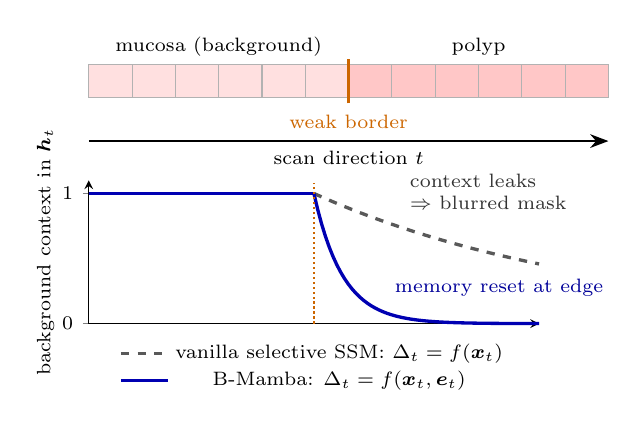
\begin{tikzpicture}[font=\scriptsize]
  % token strip
  \foreach \i in {0,...,5} {\fill[red!12, draw=gray!60] (\i*0.55,1.95) rectangle ++(0.55,0.42);}
  \foreach \i in {6,...,11} {\fill[red!22, draw=gray!60] (\i*0.55,1.95) rectangle ++(0.55,0.42);}
  \node at (1.65,2.6) {mucosa (background)};
  \node at (4.95,2.6) {polyp};
  \draw[very thick, orange!80!black] (3.3,1.88) -- (3.3,2.44);
  \node[orange!80!black, align=center] at (3.3,1.65) {weak border};
  \draw[-{Stealth}, thick] (0,1.4) -- node[below]{scan direction $t$} (6.6,1.4);
  \begin{axis}[
      at={(0,0)}, anchor=north west, yshift=0.9cm,
      width=7.3cm, height=3.4cm, scale only axis=false,
      xmin=0, xmax=12, ymin=0, ymax=1.1,
      xtick=\empty, ytick={0,1},
      ylabel={\scriptsize background context in $\vect{h}_t$},
      ylabel style={yshift=-4pt},
      legend style={font=\scriptsize, at={(0.5,-0.06)}, anchor=north, draw=none, legend columns=1, row sep=-1pt},
      axis lines=left, clip=false]
    \addplot[gray!70!black, very thick, dashed, domain=0:6, samples=2] {1};
    \addplot[gray!70!black, very thick, dashed, domain=6:12, samples=60, forget plot] {exp(-0.13*(x-6))};
    \addlegendentry{vanilla selective SSM: $\Dt_t=f(\vect{x}_t)$}
    \addplot[blue!70!black, very thick, domain=0:6, samples=2] {1};
    \addplot[blue!70!black, very thick, domain=6:12, samples=60, forget plot] {exp(-1.3*(x-6))};
    \addlegendentry{B-Mamba: $\Dt_t=f(\vect{x}_t,\vect{e}_t)$}
    \draw[orange!80!black, thick, densely dotted] (axis cs:6,0) -- (axis cs:6,1.08);
    \node[gray!40!black, align=left, anchor=south west] at (axis cs:8.3,0.80) {context leaks\\$\Rightarrow$ blurred mask};
    \node[blue!60!black, align=left, anchor=west] at (axis cs:7.9,0.28) {memory reset at edge};
  \end{axis}
\end{tikzpicture}
\caption{The problem B-Mamba addresses (conceptual sketch, not measured data). A selective SSM reads image tokens one after another and keeps a running memory $\vect{h}_t$. How fast it forgets is set by the step size $\Dt_t$. In existing vision Mamba models $\Dt_t$ depends only on the local appearance $\vect{x}_t$; at a weak border the appearance barely changes, so background context keeps flowing into the polyp region. B-Mamba also feeds an explicit boundary token $\vect{e}_t$ into $\Dt_t$, $\vect{B}_t$ and $\vect{C}_t$, so the scan can learn to reset its memory exactly at the edge. Measured step-size maps are shown in Fig.~\ref{fig:delta}.}
\label{fig:intro}
\end{figure}

\textbf{A blind spot of selective SSMs at object borders.} The power of Mamba comes from \emph{selectivity}: the step size $\Dt_t$ and the matrices $\vect{B}_t,\vect{C}_t$ are computed from the current token, so the model decides, token by token, how much of its memory to keep and what to write into it \cite{gu2023mamba}. A large $\Dt_t$ makes the model forget the past and focus on the current input; a small $\Dt_t$ makes it carry context forward. This is exactly the behavior one wants at an object border: \emph{keep context inside a region, forget it when crossing into a different one}. Yet in existing vision Mamba models \cite{zhu2024vim,liu2024vmamba,ma2024umamba,ruan2024vmunet}, these parameters are computed only from the local feature vector. At a weak border the feature vector changes very little, so the model receives almost no signal to reset its memory, and context from the mucosa ``leaks'' into the polyp (Fig.~\ref{fig:intro}). Existing boundary-aware polyp networks \cite{fang2019sfa,fan2020pranet,bui2024meganet} use edges only to re-weight features or as an extra loss; none of them uses edges to steer the \emph{dynamics} of a state space model.

\textbf{Our idea.} We make the memory of the SSM boundary-aware by construction. A parameter-free Sobel operator extracts a gradient-magnitude prior from the deepest features; this prior gates a learned high-frequency feature and is projected into a sequence of \emph{boundary tokens}. Each boundary token is fed, together with the visual token, into the projections that produce $\Dt_t$, $\vect{B}_t$ and $\vect{C}_t$. The resulting block, which we call the \emph{Boundary-Conditioned SSM} (BC-SSM), keeps the linear-time recurrence of Mamba, but every decision about \emph{remembering} and \emph{forgetting} now has direct access to where the edges are. Because the Sobel prior is a fixed, parameter-free operator rather than a learned edge detector, it cannot overfit to the color statistics of the training hospitals, which we expect to help under domain shift.

\textbf{Contributions.} The main contributions of this paper are:
\begin{enumerate}
  \item We identify that the selection mechanism of vision SSMs has no explicit access to object boundaries, and propose the Boundary-Conditioned SSM, which injects a fixed gradient prior directly into the step size and input/output matrices of the selective scan. To our knowledge, this is the first work that conditions the \emph{state dynamics} of an SSM, rather than its features or its loss, on boundary information.
  \item We give a simple theoretical analysis of the BC-SSM. We show that it strictly contains the standard selective SSM (Proposition~\ref{prop:reduction}), that the information flow between two tokens is bounded by an exponential of the accumulated step size between them (Proposition~\ref{prop:kernel}), and that positive boundary responses provably increase this ``distance'' across edges even when the appearance does not change (Proposition~\ref{prop:gating}). This links BC-SSM to edge-preserving filters such as anisotropic diffusion \cite{perona1990anisotropic}.
  \item We build B-Mamba, a complete segmentation network around the BC-SSM, and evaluate it under the standard five-dataset PraNet protocol \cite{fan2020pranet} with a leakage-checked training split, three random seeds, region and boundary metrics (Dice, IoU, MAE, Boundary-IoU \cite{cheng2021boundaryiou}, HD95), full ablations, a mechanistic analysis of the learned step sizes, and an honest computational comparison with self-attention.
\end{enumerate}

The rest of the paper is organized as follows. Section~\ref{sec:related} reviews related work. Section~\ref{sec:prelim} introduces state space models in plain terms. Section~\ref{sec:method} presents B-Mamba and its analysis. Section~\ref{sec:exp} reports experiments, Section~\ref{sec:discussion} discusses limitations, and Section~\ref{sec:conclusion} concludes.

% ==================================================================
\section{Related Work}
\label{sec:related}

\subsection{Polyp Segmentation}
Early deep models for polyp segmentation adapted general encoder--decoder networks such as U-Net \cite{ronneberger2015unet} and UNet++ \cite{zhou2018unetpp}. PraNet \cite{fan2020pranet} introduced parallel partial decoding and reverse attention, and, importantly, a common evaluation protocol: train on 1,450 images from Kvasir-SEG \cite{jha2020kvasir} and CVC-ClinicDB \cite{bernal2015clinicdb}, then test on held-out images of these two sets and on three completely unseen datasets, CVC-ColonDB \cite{tajbakhsh2016colondb}, ETIS-LaribPolypDB \cite{silva2014etis} and CVC-300 from EndoScene \cite{vazquez2017endoscene}. Later CNNs improved context selection (ACSNet \cite{zhang2020acsnet}), small-polyp detail (SANet \cite{wei2021sanet}), multi-scale differences (MSNet \cite{zhao2021msnet}) and speed (HarDNet-MSEG \cite{huang2021hardnet}). Transformer-based models brought large gains on the unseen sets: Polyp-PVT \cite{dong2023polyppvt} and SSFormer \cite{wang2022ssformer} use pyramid vision transformers \cite{wang2021pvt}, while CaraNet \cite{lou2022caranet} adds axial reverse attention for small objects.

\textbf{Boundary-aware polyp segmentation.} Because polyp borders are the hardest part to segment, many works add boundary information. SFA \cite{fang2019sfa} uses an area--boundary constraint, PraNet's reverse attention erases already-found regions to focus on borders \cite{fan2020pranet}, and MEGANet \cite{bui2024meganet} uses Laplacian edge maps to guide attention for weak boundaries. Boundary-specific losses \cite{kervadec2021boundary} and edge-detection branches \cite{xie2015hed} are also common. In all these methods the edge acts on \emph{features} (re-weighting) or on the \emph{objective} (an extra loss). B-Mamba differs in where the edge acts: it changes the \emph{state transition} of the sequence model, i.e., how information propagates through the image.

\subsection{State Space Models and Vision Mamba}
State space models describe a sequence through a hidden state that evolves linearly over time. HiPPO \cite{gu2020hippo} showed how to design the state matrix to remember long histories, S4 \cite{gu2022s4} made such models efficient, and S4D \cite{gu2022s4d} showed that a simple diagonal state matrix works well. Mamba \cite{gu2023mamba} made the SSM parameters functions of the input (``selective'') and introduced a hardware-aware parallel scan; Mamba-2 \cite{dao2024mamba2} later connected selective SSMs with linear attention \cite{katharopoulos2020linear}. Ali \emph{et al.} \cite{ali2024hidden} showed that a selective SSM can be rewritten as an implicit, data-dependent attention matrix, a view that we use in our analysis. For images, Vision Mamba \cite{zhu2024vim} scans patches in two directions and VMamba \cite{liu2024vmamba} scans in four.

\subsection{Mamba for Medical Image Segmentation}
U-Mamba \cite{ma2024umamba} inserts Mamba layers into a CNN U-Net, VM-UNet \cite{ruan2024vmunet} and VM-UNet-V2 \cite{zhang2024vmunetv2} build U-shaped networks from VMamba blocks, Mamba-UNet \cite{wang2024mambaunet} uses a pure Mamba design, Swin-UMamba \cite{liu2024swinumamba} shows the value of ImageNet pre-training, SegMamba \cite{xing2024segmamba} targets 3D volumes and LightM-UNet \cite{liao2024lightmunet} targets efficiency. For polyps, Polyp-Mamba \cite{xu2024polypmamba} and ProMamba \cite{xie2024promamba} adapt Mamba with semantic and prompt-based designs. All of these works change \emph{where} Mamba blocks are placed or \emph{how} tokens are scanned. To our knowledge, none of them changes \emph{what the selection mechanism sees}; the step size and the input/output matrices are always computed from the visual token alone.

\subsection{Conditioning and Edge-Preserving Propagation}
Feature-wise conditioning such as FiLM \cite{perez2018film} modulates activations with side information. Our approach is related in spirit but conditions the \emph{parameters of a recurrence} instead of activations. It is also related to classical edge-preserving filters: anisotropic diffusion \cite{perona1990anisotropic} lowers the diffusion rate across strong gradients, and the bilateral filter \cite{tomasi1998bilateral} down-weights neighbors with different intensities. BC-SSM can be seen as a learned, long-range, linear-time version of this idea, where the ``conductance'' between tokens is controlled by boundary-conditioned step sizes (Section~\ref{sec:theory}).

% ==================================================================
\section{Preliminaries: State Space Models in Plain Terms}
\label{sec:prelim}

\subsection{Continuous-Time State Space Models}
A state space model maps an input signal $x(t)\in\R$ to an output $y(t)\in\R$ through a hidden state $\vect{h}(t)\in\R^{N}$:
\begin{equation}
  \vect{h}'(t) = \vect{A}\,\vect{h}(t) + \vect{B}\,x(t), \qquad y(t) = \vect{C}^{\top}\vect{h}(t),
  \label{eq:ssm_cont}
\end{equation}
where $\vect{A}\in\R^{N\times N}$ is the \emph{state matrix}, and $\vect{B},\vect{C}\in\R^{N}$ are the \emph{input} and \emph{output} vectors. In simple terms, $\vect{h}(t)$ is a short ``memory'' of everything seen so far: $\vect{A}$ decides how this memory fades, $\vect{B}$ decides what is written into it, and $\vect{C}$ decides what is read out of it. Following S4D and Mamba \cite{gu2022s4d,gu2023mamba}, we use a diagonal $\vect{A}$ with negative entries, $\vect{A}=\mathrm{diag}(a_1,\dots,a_N)$, $a_n<0$, so the memory is stable and each of its $N$ slots fades at its own rate.

\subsection{Discretization}
Images are discrete, so \eqref{eq:ssm_cont} is converted to a recurrence using a step size $\Dt>0$. With the zero-order-hold (ZOH) rule,
\begin{align}
  \bar{\vect{A}} &= \exp(\Dt\vect{A}), \label{eq:zoh_A}\\
  \bar{\vect{B}} &= (\Dt\vect{A})^{-1}\big(\exp(\Dt\vect{A})-\vect{I}\big)\,\Dt\vect{B} \;\approx\; \Dt\vect{B}, \label{eq:zoh_B}
\end{align}
and the model becomes
\begin{equation}
  \vect{h}_t = \bar{\vect{A}}\,\vect{h}_{t-1} + \bar{\vect{B}}\,x_t, \qquad y_t = \vect{C}^{\top}\vect{h}_t + D\,x_t,
  \label{eq:ssm_disc}
\end{equation}
where $D$ is a skip connection. Like Mamba, we use the first-order approximation $\bar{\vect{B}}\approx\Dt\vect{B}$ in \eqref{eq:zoh_B}. Because $a_n<0$, each entry of $\bar{\vect{A}}=\exp(\Dt\vect{A})$ lies in $(0,1)$. \emph{The step size is therefore a forgetting knob}: a small $\Dt$ gives $\bar{\vect{A}}\approx\vect{I}$ (remember almost everything), and a large $\Dt$ gives $\bar{\vect{A}}\approx\vect{0}$ (forget the past and focus on the current input).

\subsection{Selective State Space Models (Mamba)}
In S4 the parameters $(\Dt,\vect{B},\vect{C})$ are the same for every position. Mamba \cite{gu2023mamba} makes them depend on the input, which lets the model choose, token by token, what to keep. For a $D$-channel input sequence $\vect{u}_1,\dots,\vect{u}_L\in\R^{D}$, the selective SSM (S6) computes
\begin{equation}
  \vect{B}_t = \vect{W}_B\vect{u}_t,\quad \vect{C}_t = \vect{W}_C\vect{u}_t,\quad \Dt_t = \softplus(\vect{W}_\Dt\vect{u}_t + \vect{b}_\Dt),
  \label{eq:s6}
\end{equation}
with $\vect{B}_t,\vect{C}_t\in\R^{N}$ shared across channels and $\Dt_t\in\R^{D}_{>0}$ giving one step size per channel. Each channel $d$ then runs its own recurrence \eqref{eq:ssm_disc} with $\bar{\vect{A}}_{t,d}=\exp(\Dt_{t,d}\vect{A}_d)$ and $\bar{\vect{B}}_{t,d}=\Dt_{t,d}\vect{B}_t$. Since the recurrence is linear in $\vect{h}$, it can be computed with a parallel scan in $O(L)$ work, which is the source of Mamba's linear complexity.

\subsection{The Unrolled View: SSMs as Implicit Attention}
Unrolling \eqref{eq:ssm_disc} for one channel $d$ gives \cite{ali2024hidden,dao2024mamba2}
\begin{equation}
  y_{t,d} = \sum_{s=1}^{t} \underbrace{\vect{C}_t^{\top}\Big(\prod_{k=s+1}^{t}\bar{\vect{A}}_{k,d}\Big)\bar{\vect{B}}_{s,d}}_{\alpha^{(d)}_{t,s}}\; u_{s,d} \;+\; D_d\,u_{t,d}.
  \label{eq:unrolled}
\end{equation}
The coefficient $\alpha^{(d)}_{t,s}$ tells us how much token $s$ influences token $t$, just like an attention weight. It contains three parts: what token $s$ wrote ($\bar{\vect{B}}_{s}$, a ``key''), what token $t$ reads ($\vect{C}_t$, a ``query''), and how much of the message survived the trip from $s$ to $t$ (the product of $\bar{\vect{A}}$, a ``decay''). This view makes it clear that \emph{the step sizes between two tokens control how much they can talk to each other}. We use it in Section~\ref{sec:theory}.

% ==================================================================
\section{Method}
\label{sec:method}

\begin{figure*}[t]
\centering
\resizebox{\textwidth}{!}{%
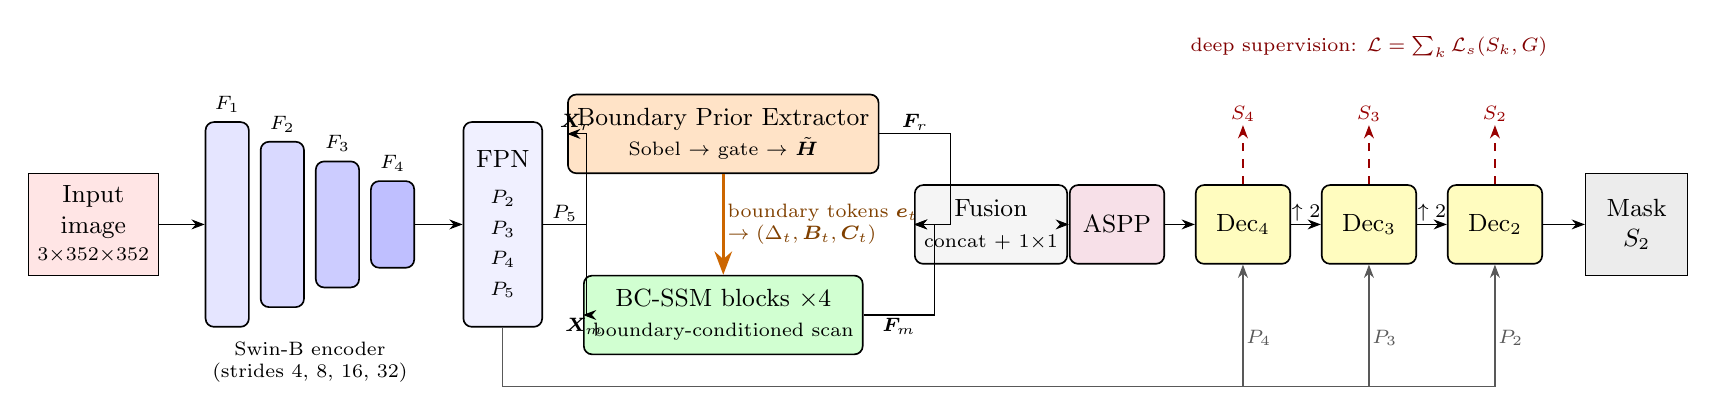
\begin{tikzpicture}[font=\small, >=Stealth,
  blk/.style={draw, rounded corners=3pt, minimum height=1.0cm, minimum width=1.6cm, align=center, fill=#1, line width=0.6pt},
  blk/.default=gray!8,
  lab/.style={font=\scriptsize, inner sep=1pt}]
  % input image
  \node[draw, minimum size=1.3cm, fill=red!10, align=center] (img) at (0,0) {Input\\image\\[-1pt]\scriptsize $3{\times}352{\times}352$};
  % encoder stages
  \node[blk=blue!10, minimum height=2.6cm, minimum width=0.55cm] (e1) at (1.7,0) {};
  \node[blk=blue!15, minimum height=2.1cm, minimum width=0.55cm] (e2) at (2.4,0) {};
  \node[blk=blue!20, minimum height=1.6cm, minimum width=0.55cm] (e3) at (3.1,0) {};
  \node[blk=blue!25, minimum height=1.1cm, minimum width=0.55cm] (e4) at (3.8,0) {};
  \node[lab, above=2pt of e1] {$F_1$}; \node[lab, above=2pt of e2] {$F_2$};
  \node[lab, above=2pt of e3] {$F_3$}; \node[lab, above=2pt of e4] {$F_4$};
  \node[font=\scriptsize, align=center] at (2.75,-1.75) {Swin-B encoder\\(strides 4, 8, 16, 32)};
  \draw[->] (img) -- (e1);
  % FPN
  \node[blk=blue!6, minimum height=2.6cm, minimum width=1.0cm] (fpn) at (5.2,0) {FPN\\[2pt]\scriptsize$P_2$\\\scriptsize$P_3$\\\scriptsize$P_4$\\\scriptsize$P_5$};
  \draw[->] (e4) -- (fpn);
  % two branches at P5
  \node[blk=orange!22, minimum width=2.7cm] (bpe) at (8.0,1.15) {Boundary Prior Extractor\\\scriptsize Sobel $\rightarrow$ gate $\rightarrow$ $\tilde{\vect{H}}$};
  \node[blk=green!18, minimum width=2.7cm] (ssm) at (8.0,-1.15) {BC-SSM blocks $\times4$\\\scriptsize boundary-conditioned scan};
  \draw[->] (fpn.east) -- node[lab, above]{$P_5$} ++(0.55,0) coordinate (br) |- node[lab, pos=0.78, above]{$\vect{X}_r$} (bpe.west);
  \draw[->] (br) |- node[lab, pos=0.78, below]{$\vect{X}_m$} (ssm.west);
  \draw[->, very thick, orange!80!black] (bpe.south) -- node[lab, right, align=left, text=orange!50!black]{boundary tokens $\vect{e}_t$\\$\rightarrow(\Dt_t,\vect{B}_t,\vect{C}_t)$} (ssm.north);
  % fusion
  \node[blk] (fus) at (11.4,0) {Fusion\\\scriptsize concat + $1{\times}1$};
  \draw[->] (bpe.east) -- node[lab, above]{$\vect{F}_r$} ++(0.9,0) |- (fus.west);
  \draw[->] (ssm.east) -- node[lab, below]{$\vect{F}_m$} ++(0.9,0) |- (fus.west);
  \node[blk=purple!12, minimum width=1.2cm] (aspp) at (13.0,0) {ASPP};
  \draw[->] (fus) -- (aspp);
  % decoder
  \node[blk=yellow!25, minimum width=1.2cm] (d4) at (14.6,0) {Dec$_4$};
  \node[blk=yellow!25, minimum width=1.2cm] (d3) at (16.2,0) {Dec$_3$};
  \node[blk=yellow!25, minimum width=1.2cm] (d2) at (17.8,0) {Dec$_2$};
  \node[draw, minimum size=1.3cm, fill=gray!15, align=center] (out) at (19.6,0) {Mask\\$S_2$};
  \draw[->] (aspp) -- (d4); \draw[->] (d4) -- node[lab, above]{$\uparrow2$}(d3); \draw[->] (d3) -- node[lab, above]{$\uparrow2$}(d2); \draw[->] (d2) -- (out);
  % laterals
  \draw[gray!70!black] (fpn.south) -- ++(0,-0.75) coordinate (lb) -- (lb -| d2);
  \draw[->, gray!70!black] (lb -| d4) -- node[lab, right, pos=0.4]{$P_4$} (d4.south);
  \draw[->, gray!70!black] (lb -| d3) -- node[lab, right, pos=0.4]{$P_3$} (d3.south);
  \draw[->, gray!70!black] (lb -| d2) -- node[lab, right, pos=0.4]{$P_2$} (d2.south);
  % deep supervision
  \draw[->, dashed, red!60!black] (d4.north) -- ++(0,0.75) node[lab, above]{$S_4$};
  \draw[->, dashed, red!60!black] (d3.north) -- ++(0,0.75) node[lab, above]{$S_3$};
  \draw[->, dashed, red!60!black] (d2.north) -- ++(0,0.75) node[lab, above]{$S_2$};
  \node[font=\scriptsize, red!50!black] at (16.2,2.25) {deep supervision: $\mathcal{L}=\sum_{k}\mathcal{L}_{s}(S_k,G)$};
\end{tikzpicture}}
\caption{Overview of B-Mamba. A Swin-B encoder and a feature pyramid network (FPN) produce multi-scale features $P_2$--$P_5$. At the coarsest level, two parallel branches process $P_5$: the Boundary Prior Extractor (BPE) computes a Sobel prior and a boundary-gated texture feature, and the BC-SSM branch models global context with a selective scan whose parameters are conditioned on the boundary tokens produced by the BPE (orange arrow). The two outputs are fused and decoded by an ASPP module and a three-stage progressive decoder with lateral FPN connections. Side outputs $S_4,S_3,S_2$ are supervised during training; only $S_2$ is used at test time.}
\label{fig:arch}
\end{figure*}

\subsection{Overview}
Fig.~\ref{fig:arch} shows the full network. Given an image $\vect{I}\in\R^{3\times H\times W}$ ($H=W=352$), a hierarchical encoder extracts features at four scales. A feature pyramid network mixes them so that every scale carries both detail and semantics. At the coarsest scale, where each token covers a $32\times32$ patch and the whole polyp is visible to the model, we place two complementary branches: a \emph{Boundary Prior Extractor} that finds where edges are, and a stack of \emph{Boundary-Conditioned SSM} blocks that model global context while using those edges to control their memory. A decoder then recovers full resolution. We now describe each part, using the same symbols as our released code.

\subsection{Hierarchical Encoder and Feature Pyramid}
We use a Swin-B Transformer \cite{liu2021swin} pre-trained on ImageNet as the encoder. It outputs $F_i\in\R^{C_i\times\frac{H}{2^{i+1}}\times\frac{W}{2^{i+1}}}$ for $i=1,\dots,4$, with $C_i\in\{128,256,512,1024\}$ and spatial strides $\{4,8,16,32\}$. A feature pyramid network \cite{lin2017fpn} maps these to $P_{i+1}\in\R^{256\times\frac{H}{2^{i+1}}\times\frac{W}{2^{i+1}}}$. The coarsest map $P_5$ has size $11\times11$ for a $352\times352$ input, so the BC-SSM operates on $L=121$ tokens. $P_5$ is projected into two separate $512$-channel inputs, $\vect{X}_r=\phi_r(P_5)$ for the boundary branch and $\vect{X}_m=\phi_m(P_5)$ for the SSM branch, where each $\phi$ is a $1\times1$ convolution followed by batch normalization and ReLU.

\subsection{Boundary Prior Extractor (BPE)}
\label{sec:bpe}
The BPE has two jobs: produce a better local feature for the final prediction, and produce the boundary tokens that will steer the SSM.

\textbf{Sobel gradient prior.} We first average the feature channels into a single map, $\bar{X}=\frac{1}{C}\sum_{c=1}^{C}\vect{X}_r[c]\in\R^{h\times w}$, and apply the classical Sobel operator \cite{sobel1990isotropic}:
\begin{equation}
  K_x=\begin{bmatrix}-1&0&1\\-2&0&2\\-1&0&1\end{bmatrix},\quad K_y=K_x^{\top},\quad
  \begin{aligned} G_x &= K_x * \bar{X},\\ G_y &= K_y * \bar{X},\end{aligned}
  \label{eq:sobel}
\end{equation}
\begin{equation}
  M = \sqrt{G_x^{2}+G_y^{2}+\epsilon},\qquad E=\sigma(M)\in\big[\tfrac12,\,1\big),
  \label{eq:edge}
\end{equation}
where $*$ is 2D convolution, $\sigma$ is the logistic sigmoid and $\epsilon=10^{-6}$ keeps the square root differentiable. The kernels $K_x,K_y$ are fixed (not learned). $E$ equals $\tfrac12$ in perfectly flat regions and approaches $1$ at strong gradients. We apply Sobel to deep features rather than to the raw image on purpose: in the raw image, the strongest gradients usually come from specular highlights and vessel patterns, whereas in deep features they tend to mark changes in \emph{semantic} content.

\textbf{Boundary-gated texture feature.} In parallel, a small high-frequency network extracts local texture:
\begin{equation}
  \vect{H}=\rho\big(\mathrm{Conv}^{3\times3}_{\text{dil}=2}\big(\rho(\mathrm{Conv}^{3\times3}(\vect{X}_r))\big)\big),
  \label{eq:hf}
\end{equation}
where $\rho(\cdot)$ denotes batch normalization followed by ReLU. The Sobel prior then acts as a soft spatial gate:
\begin{equation}
  \tilde{\vect{H}} = \vect{H}\odot(1+E),
  \label{eq:gate}
\end{equation}
with $E$ broadcast over channels. Because $E\in[\frac12,1)$, the gate amplifies features at edges by up to $4/3$ relative to flat regions while never zeroing out any location. The output of the boundary branch is
\begin{equation}
  \vect{F}_r = \rho\big(\mathrm{Conv}^{1\times1}([\tilde{\vect{H}};E])\big)\in\R^{512\times h\times w},
  \label{eq:Fr}
\end{equation}
where $[\cdot;\cdot]$ is channel concatenation.

\textbf{Boundary tokens.} The boundary-gated feature $\tilde{\vect{H}}$ is projected to the inner width of the SSM, $D=1024$, and flattened in raster order:
\begin{equation}
  \vect{e} = \mathrm{Flatten}\big(\mathrm{Conv}^{1\times1}(\tilde{\vect{H}})\big)\in\R^{L\times D},\qquad L=hw.
  \label{eq:tokens}
\end{equation}
The $t$-th row $\vect{e}_t$ is the boundary token for position $t$. It combines a fixed, appearance-independent cue ($E$) with learned local texture ($\vect{H}$), so the SSM receives both ``\emph{is there an edge here?}'' and ``\emph{what kind of edge is it?}''.

\subsection{Boundary-Conditioned State Space Block (BC-SSM)}
\label{sec:bcssm}

\begin{figure}[t]
\centering
\resizebox{\linewidth}{!}{%
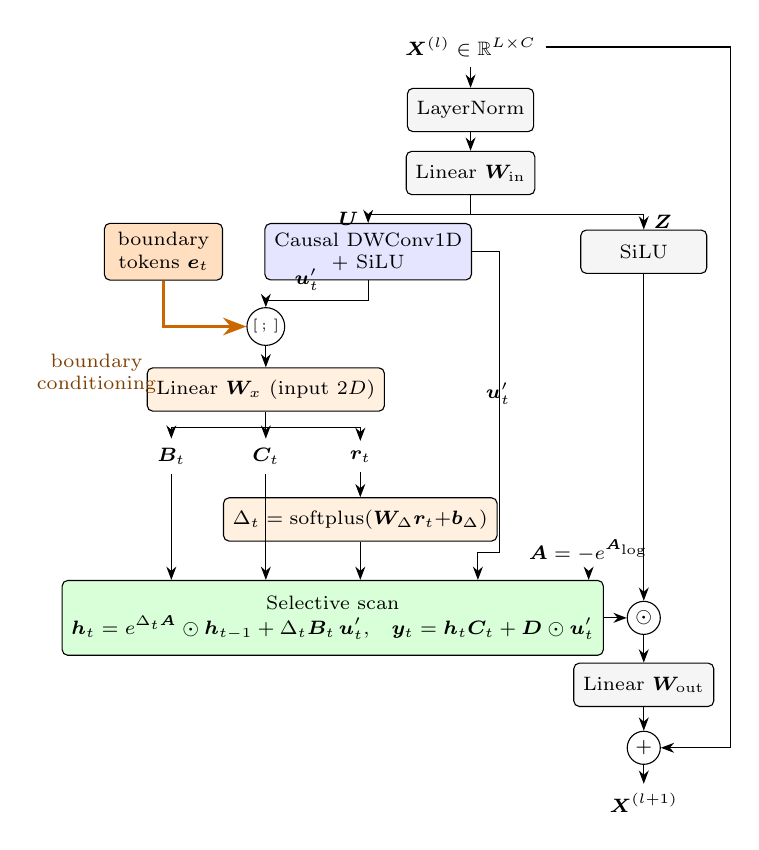
\begin{tikzpicture}[font=\scriptsize, >=Stealth,
  op/.style={draw, rounded corners=2pt, fill=#1, minimum height=0.55cm, minimum width=1.6cm, align=center},
  op/.default=gray!8,
  circ/.style={draw, circle, inner sep=1pt, minimum size=0.42cm, fill=white}]
  \node (in) at (2.2,0.2) {$\vect{X}^{(l)}\in\R^{L\times C}$};
  \node[op] (ln) at (2.2,-0.6) {LayerNorm};
  \node[op] (win) at (2.2,-1.4) {Linear $\vect{W}_{\text{in}}$};
  \node[op=blue!10, minimum width=2.0cm] (conv) at (0.9,-2.4) {Causal DWConv1D\\$+$ SiLU};
  \node[op=orange!25, minimum width=1.5cm] (e) at (-1.7,-2.4) {boundary\\tokens $\vect{e}_t$};
  \node[op] (zs) at (4.4,-2.4) {SiLU};
  \node[circ] (cat) at (-0.4,-3.35) {\tiny $[\,;\,]$};
  \node[op=orange!12, minimum width=2.4cm] (wx) at (-0.4,-4.15) {Linear $\vect{W}_x$ (input $2D$)};
  \node (B) at (-1.6,-5.0) {$\vect{B}_t$};
  \node (C) at (-0.4,-5.0) {$\vect{C}_t$};
  \node (r) at (0.8,-5.0) {$\vect{r}_t$};
  \node[op=orange!12, minimum width=2.1cm] (dt) at (0.8,-5.8) {$\Dt_t=\softplus(\vect{W}_\Dt\vect{r}_t{+}\vect{b}_\Dt)$};
  \node[op=green!15, minimum width=5.2cm, minimum height=0.95cm] (scan) at (0.45,-7.05) {Selective scan\\[1pt]$\vect{h}_t=e^{\Dt_t\vect{A}}\odot\vect{h}_{t-1}+\Dt_t\vect{B}_t\,\vect{u}'_t$,\quad $\vect{y}_t=\vect{h}_t\vect{C}_t+\vect{D}\odot\vect{u}'_t$};
  \node (A) at (3.7,-6.2) {$\vect{A}=-e^{\vect{A}_{\log}}$};
  \node[circ] (mul) at (4.4,-7.05) {$\odot$};
  \node[op] (wout) at (4.4,-7.9) {Linear $\vect{W}_{\text{out}}$};
  \node[circ] (add) at (4.4,-8.7) {$+$};
  \node (out) at (4.4,-9.4) {$\vect{X}^{(l+1)}$};
  % edges
  \draw[->] (in) -- (ln); \draw[->] (ln) -- (win);
  \draw[->] (win.south) -- ++(0,-0.25) -| node[pos=0.75,left]{$\vect{U}$} (conv.north);
  \draw[->] (win.south) -- ++(0,-0.25) -| node[pos=0.75,right]{$\vect{Z}$} (zs.north);
  \draw[->] (conv.south) -- ++(0,-0.25) -| node[pos=0.3, above]{$\vect{u}'_t$} (cat.north);
  \draw[->] (conv.east) -- ++(0.35,0) |- ($(scan.north east)+(-1.6,0.35)$) -- ++(0,-0.35);
  \node at (2.55,-4.2) {$\vect{u}'_t$};
  \draw[->, very thick, orange!80!black] (e.south) |- (cat.west);
  \draw[->] (cat) -- (wx);
  \draw[->] (wx.south) -- ++(0,-0.2) -| (B.north);
  \draw[->] (wx.south) -- (C.north);
  \draw[->] (wx.south) -- ++(0,-0.2) -| (r.north);
  \draw[->] (r) -- (dt);
  \draw[->] (B.south) -- (B.south |- scan.north);
  \draw[->] (C.south) -- (C.south |- scan.north);
  \draw[->] (dt.south) -- (dt.south |- scan.north);
  \draw[->] (A.south) -- (A.south |- scan.north);
  \draw[->] (scan.east) -- (mul.west);
  \draw[->] (zs.south) -- (mul.north);
  \draw[->] (mul) -- (wout); \draw[->] (wout) -- (add); \draw[->] (add) -- (out);
  \draw[->] (in.east) -- (5.5,0.2) |- (add.east);
  \node[orange!50!black, align=center] at (-2.55,-3.95) {boundary\\conditioning};
\end{tikzpicture}}
\caption{The Boundary-Conditioned SSM block. Orange parts are new compared with a standard Mamba block: the boundary token $\vect{e}_t$ is concatenated with the visual token $\vect{u}'_t$ before the projection that produces the step size $\Dt_t$ and the matrices $\vect{B}_t,\vect{C}_t$. Everything else, including the linear-time scan, is unchanged.}
\label{fig:block}
\end{figure}

The SSM branch first applies a $1\times1$ convolution to $\vect{X}_m$ and flattens it in raster (row-major) order into a sequence $\vect{X}^{(0)}\in\R^{L\times C}$ with $C=512$. It then applies four BC-SSM blocks (Fig.~\ref{fig:block}). Block $l$ maps $\vect{X}^{(l)}$ to $\vect{X}^{(l+1)}$ as follows.

\textbf{Step 1 -- input projection and local mixing.}
\begin{align}
  [\vect{U};\vect{Z}] &= \LN(\vect{X}^{(l)})\,\vect{W}_{\text{in}}, \qquad \vect{U},\vect{Z}\in\R^{L\times D}, \label{eq:inproj}\\
  \vect{U}' &= \SiLU\big(\mathrm{DWConv1D}_{k=4}(\vect{U})\big), \label{eq:conv}
\end{align}
where $D=2C=1024$, $\mathrm{DWConv1D}_{k=4}$ is a causal depth-wise 1D convolution of width 4, and $\vect{Z}$ is a gate branch.

\textbf{Step 2 -- boundary-conditioned selection (the key change).} For each position $t$ we form a joint descriptor from the visual token $\vect{u}'_t$ and the boundary token $\vect{e}_t$, and compute all selective parameters from it:
\begin{align}
  \vect{q}_t &= [\,\vect{u}'_t\,;\,\vect{e}_t\,]\in\R^{2D}, \label{eq:joint}\\
  [\,\vect{B}_t;\,\vect{C}_t;\,\vect{r}_t\,] &= \vect{W}_x\,\vect{q}_t,\qquad \vect{W}_x\in\R^{(2N+D)\times 2D}, \label{eq:xproj}\\
  \Dt_t &= \softplus\big(\vect{W}_\Dt\,\vect{r}_t + \vect{b}_\Dt\big)\in\R^{D}_{>0}, \label{eq:delta}
\end{align}
with state size $N=16$. Splitting $\vect{W}_x=[\vect{W}_x^{u}\;\vect{W}_x^{e}]$ into the columns that act on $\vect{u}'_t$ and on $\vect{e}_t$ makes the effect of the boundary explicit:
\begin{equation}
  \begin{aligned}
  \vect{B}_t &= \underbrace{\vect{W}_B^{u}\vect{u}'_t}_{\text{appearance}} + \underbrace{\vect{W}_B^{e}\vect{e}_t}_{\text{boundary}}, \qquad
  \vect{C}_t = \vect{W}_C^{u}\vect{u}'_t + \vect{W}_C^{e}\vect{e}_t,\\
  \Dt_t &= \softplus\big(\vect{G}\,\vect{u}'_t + \vect{Q}\,\vect{e}_t + \vect{b}_\Dt\big),
  \end{aligned}
  \label{eq:split}
\end{equation}
where $\vect{G}=\vect{W}_\Dt\vect{W}_r^{u}$ and $\vect{Q}=\vect{W}_\Dt\vect{W}_r^{e}$ are the combined linear maps from each input to the step size. In words: \emph{the boundary token directly shifts what the scan writes ($\vect{B}_t$), what it reads ($\vect{C}_t$) and how fast it forgets ($\Dt_t$)}.

\textbf{Step 3 -- discretization and selective scan.} With a learned diagonal state matrix $\vect{A}=-\exp(\vect{A}_{\log})\in\R^{D\times N}$ (initialized as $a_{d,n}=-n$, the S4D-real initialization \cite{gu2022s4d}), each channel $d$ runs
\begin{align}
  \bar{\vect{A}}_{t,d} &= \exp(\Dt_{t,d}\,\vect{A}_d), \qquad \bar{\vect{B}}_{t,d}=\Dt_{t,d}\,\vect{B}_t, \label{eq:disc_bc}\\
  \vect{h}_{t,d} &= \bar{\vect{A}}_{t,d}\odot\vect{h}_{t-1,d} + \bar{\vect{B}}_{t,d}\,u'_{t,d}, \label{eq:scan_bc}\\
  y_{t,d} &= \vect{C}_t^{\top}\vect{h}_{t,d} + D_d\,u'_{t,d}, \label{eq:out_bc}
\end{align}
with $\vect{h}_{0,d}=\vect{0}$ and a learned skip vector $\vect{D}$ (initialized to ones).

\textbf{Step 4 -- gating and residual.}
\begin{equation}
  \vect{X}^{(l+1)} = \big(\vect{Y}\odot\SiLU(\vect{Z})\big)\vect{W}_{\text{out}} + \vect{X}^{(l)}.
  \label{eq:outproj}
\end{equation}
After the last block, a LayerNorm, a reshape back to $h\times w$ and a $1\times1$ convolution give the global-context feature $\vect{F}_m\in\R^{512\times h\times w}$. Algorithm~\ref{alg:bcssm} summarizes the block.

\begin{algorithm}[t]
\caption{Forward pass of one BC-SSM block}
\label{alg:bcssm}
\begin{algorithmic}[1]
\Require visual tokens $\vect{X}\in\R^{L\times C}$, boundary tokens $\vect{e}\in\R^{L\times D}$
\State $[\vect{U};\vect{Z}]\gets\LN(\vect{X})\vect{W}_{\text{in}}$;\; $\vect{U}'\gets\SiLU(\mathrm{DWConv1D}(\vect{U}))$
\State $\vect{Q}_{\text{in}}\gets[\vect{U}';\vect{e}]$ \Comment{boundary conditioning}
\State $[\vect{B};\vect{C};\vect{R}]\gets\vect{Q}_{\text{in}}\vect{W}_x^{\top}$;\; $\Dt\gets\softplus(\vect{R}\vect{W}_\Dt^{\top}+\vect{b}_\Dt)$
\State $\vect{A}\gets-\exp(\vect{A}_{\log})$;\; $\vect{h}\gets\vect{0}\in\R^{D\times N}$
\For{$t=1$ to $L$} \Comment{parallel scan in practice}
  \State $\vect{h}\gets\exp(\Dt_t\otimes\vect{A})\odot\vect{h}+(\Dt_t\otimes\vect{B}_t)\odot(\vect{u}'_t\otimes\vect{1}_N)$
  \State $\vect{y}_t\gets\vect{h}\,\vect{C}_t+\vect{D}\odot\vect{u}'_t$
\EndFor
\State \Return $(\vect{Y}\odot\SiLU(\vect{Z}))\vect{W}_{\text{out}}+\vect{X}$
\end{algorithmic}
\end{algorithm}

\subsection{Theoretical Analysis}
\label{sec:theory}
We now explain, with three short propositions, \emph{why} conditioning the selective parameters on boundaries is a principled change and not just extra input features. We analyze one channel $d$ and drop the index $d$ where it is clear. Let $a_{\min}=\min_n |a_{d,n}|>0$ denote the slowest decay rate of the channel.

\begin{proposition}[BC-SSM strictly contains S6]
\label{prop:reduction}
If $\vect{W}_x^{e}=\vect{0}$, or if $\vect{e}_t=\vect{0}$ for all $t$, the BC-SSM block \eqref{eq:inproj}--\eqref{eq:outproj} is exactly a Mamba (S6) block with selective parameters \eqref{eq:s6}. Hence every function computed by an S6 block can also be computed by a BC-SSM block.
\end{proposition}
\begin{IEEEproof}
Setting the boundary columns to zero in \eqref{eq:split} gives $\vect{B}_t=\vect{W}_B^{u}\vect{u}'_t$, $\vect{C}_t=\vect{W}_C^{u}\vect{u}'_t$ and $\Dt_t=\softplus(\vect{G}\vect{u}'_t+\vect{b}_\Dt)$, which is \eqref{eq:s6}. All other operations are identical.
\end{IEEEproof}
This guarantees that adding the boundary path can never reduce the representational power of the block; the optimizer can always fall back to plain Mamba. It also means that our ablation without boundaries (feeding $\vect{e}_t=\vect{0}$) is an exact S6 baseline with the same number of parameters.

\begin{definition}[Accumulated step size]
For tokens $s<t$ in channel $d$, the accumulated step size is $\tau(s,t)=\sum_{k=s+1}^{t}\Dt_{k}$.
\end{definition}

\begin{proposition}[Step sizes act as a learned distance]
\label{prop:kernel}
For the implicit attention weight $\alpha_{t,s}$ in \eqref{eq:unrolled},
\begin{equation}
  |\alpha_{t,s}| \;\le\; \Dt_{s}\,\|\vect{B}_s\|_2\,\|\vect{C}_t\|_2\;\exp\!\big(-a_{\min}\,\tau(s,t)\big).
  \label{eq:kernel_bound}
\end{equation}
\end{proposition}
\begin{IEEEproof}
Because $\vect{A}_d$ is diagonal, the product of transitions is $\prod_{k=s+1}^{t}\exp(\Dt_{k}\vect{A}_d)=\exp\big(\tau(s,t)\vect{A}_d\big)$, a diagonal matrix with entries $\exp(-|a_{n}|\tau(s,t))\le\exp(-a_{\min}\tau(s,t))$. Hence $\alpha_{t,s}=\Dt_{s}\,\vect{C}_t^{\top}\exp(\tau(s,t)\vect{A}_d)\vect{B}_s$, and the Cauchy--Schwarz inequality together with the bound on the largest diagonal entry gives \eqref{eq:kernel_bound}.
\end{IEEEproof}
In plain words: \emph{two tokens can only exchange information if the step sizes between them add up to a small number}. The accumulated step size $\tau(s,t)$ behaves like a distance that the network learns. If the scan takes a large step anywhere between $s$ and $t$, the influence of $s$ on $t$ shrinks exponentially, no matter how similar the two tokens look.

\begin{proposition}[Boundary evidence lengthens the distance across edges]
\label{prop:gating}
Compare a BC-SSM channel with the same channel when the boundary input is removed (the S6 model of Proposition~\ref{prop:reduction}), for the same visual tokens. Write $z_k=\vect{g}^{\top}\vect{u}'_k+b$ for the appearance part of the pre-activation of $\Dt_k$, and $\gamma_k=\vect{q}^{\top}\vect{e}_k$ for its boundary part, where $\vect{g}^{\top}$ and $\vect{q}^{\top}$ are the $d$-th rows of $\vect{G}$ and $\vect{Q}$. If $\gamma_k\ge0$ for every token $k$ between $s$ and $t$, then
\begin{equation}
  \tau^{\text{BC}}(s,t) \;\ge\; \tau^{\text{S6}}(s,t) + \sum_{k=s+1}^{t}\sigma(z_k)\,\gamma_k ,
  \label{eq:gating}
\end{equation}
and therefore the bound \eqref{eq:kernel_bound} on the influence of $s$ on $t$ is multiplied by at most $\exp\!\big(-a_{\min}\sum_{k}\sigma(z_k)\gamma_k\big)\le1$.
\end{proposition}
\begin{IEEEproof}
The softplus function is convex with derivative $\sigma$. By convexity, $\softplus(z+\gamma)\ge\softplus(z)+\gamma\,\sigma(z)$ for all $z,\gamma\in\R$. Applying this to each term $\Dt_k^{\text{BC}}=\softplus(z_k+\gamma_k)$ and summing over $k$ gives \eqref{eq:gating}. Substituting into \eqref{eq:kernel_bound} gives the second statement.
\end{IEEEproof}

\begin{remark}[What the propositions mean for weak borders]
The extra distance in \eqref{eq:gating} depends on the boundary response $\gamma_k$, \emph{not} on how much the appearance changes. Consider a weak border where the visual tokens on both sides are almost identical, so the appearance terms $z_k$ hardly change and a plain S6 model has no reason to take a large step. In BC-SSM, as long as the boundary token at the border produces $\gamma_k>0$, the scan takes a larger step exactly there, and the leakage of mucosa context into the polyp is suppressed exponentially. The sign of $\vect{q}$ is learned per channel, so some channels can also learn the opposite behavior (carrying context \emph{across} an edge, e.g., when an edge is caused by a specular highlight inside a polyp). B-Mamba thus learns an \emph{edge-aware, long-range} propagation rule, a learned counterpart of anisotropic diffusion \cite{perona1990anisotropic}, where the conductance between neighbors drops at strong gradients. Because $\vect{B}_t$ and $\vect{C}_t$ are also conditioned, boundary tokens additionally change \emph{what} is written to and read from memory, in the ``key/query'' sense of \eqref{eq:unrolled}. We test these predictions directly in Section~\ref{sec:delta}.
\end{remark}

\begin{proposition}[Complexity]
\label{prop:complexity}
A BC-SSM block on $L$ tokens costs $O\big(L\,(CD + D^{2} + DN)\big)$ operations and keeps a state of fixed size $D\times N$, independent of $L$. Compared with an S6 block of the same width, boundary conditioning adds $L\,D\,(2N+D)$ multiply--accumulates (MACs) and $D\,(2N+D)$ parameters per block. A self-attention block of width $C$ costs $O(L^{2}C + LC^{2})$.
\end{proposition}
\begin{IEEEproof}
The projections $\vect{W}_{\text{in}}$, $\vect{W}_x$, $\vect{W}_\Dt$ and $\vect{W}_{\text{out}}$ cost $L\cdot C\cdot2D$, $L\cdot2D\cdot(2N+D)$, $L\cdot D^2$ and $L\cdot DC$ MACs; the convolution costs $O(LD)$ and the scan $O(LDN)$. In S6 the input of $\vect{W}_x$ has size $D$ instead of $2D$, which gives the stated difference. The attention cost follows from the $L\times L$ score matrix.
\end{IEEEproof}
For our widths ($C=512$, $D=1024$, $N=16$) this amounts to $4.33$\,M extra parameters for the four blocks plus $0.53$\,M for the boundary-token projection, i.e., \BCparams\,M (4.0\%) and \BCmacs\,GMACs (1.1\%) of the full network. Table~\ref{tab:scaling} shows how BC-SSM and attention scale with resolution.

\subsection{Fusion and Progressive Decoder}
The local boundary feature and the global context feature are fused by $\vect{F}=\rho\big(\mathrm{Conv}^{1\times1}([\vect{F}_r;\vect{F}_m])\big)$. An atrous spatial pyramid pooling (ASPP) module \cite{chen2018deeplab} with dilation rates $\{1,6,12,18\}$ and global average pooling enlarges the receptive field and reduces $\vect{F}$ to 256 channels, giving $\vect{D}_5$. A three-stage progressive decoder then restores resolution. For $k=4,3,2$:
\begin{equation}
  \vect{D}_k = \rho\big(\mathrm{Conv}^{3\times3}\big([\,\mathrm{Up}(\vect{D}_{k+1});\;\lambda_k(P_k)\,]\big)\big),
  \label{eq:decoder}
\end{equation}
where $\mathrm{Up}$ is bilinear upsampling to the size of $P_k$, $\lambda_k$ is a $1\times1$ convolution with ReLU that reduces $P_k$ to $\{128,64,32\}$ channels, and $\vect{D}_k$ has $\{128,64,32\}$ channels. A $1\times1$ convolution on each $\vect{D}_k$ gives a side prediction $S_k$, which is bilinearly upsampled to $352\times352$.

\subsection{Training Objective with Deep Supervision}
Each side output is supervised with the structure loss of PraNet \cite{fan2020pranet,wei2020f3net}, which stresses hard pixels near the border. Let $G\in\{0,1\}^{H\times W}$ be the ground truth and $p=\sigma(S_k)$ the predicted probability. The pixel weight
\begin{equation}
  w_{ij} = 1 + 5\,\big|\,(\mathrm{AvgPool}_{31\times31}G)_{ij} - G_{ij}\,\big|
  \label{eq:weight}
\end{equation}
is large near boundaries, where the local average differs from the pixel's own label. The weighted IoU loss is
\begin{equation}
  \mathcal{L}^{w}_{\text{IoU}} = 1-\frac{\sum_{ij}w_{ij}\,p_{ij}G_{ij}+1}{\sum_{ij}w_{ij}\,(p_{ij}+G_{ij}-p_{ij}G_{ij})+1},
  \label{eq:wiou}
\end{equation}
and the structure loss is $\mathcal{L}_{s}=\mathcal{L}_{\text{BCE}}+\mathcal{L}^{w}_{\text{IoU}}$, where, as in the reference PraNet implementation, the binary cross-entropy term is averaged uniformly over pixels. Following deep supervision \cite{lee2015dsn}, the total loss is
\begin{equation}
  \mathcal{L} = \sum_{k\in\{2,3,4\}} \mathcal{L}_{s}\big(S_k,\,G\big).
  \label{eq:total}
\end{equation}
At inference, only $S_2$ is used, so the side heads add no test-time cost.

% ==================================================================
\section{Experiments}
\label{sec:exp}

\subsection{Datasets and Protocol}
We follow the widely used protocol of PraNet \cite{fan2020pranet} (Table~\ref{tab:datasets}). The training set contains 900 images from Kvasir-SEG \cite{jha2020kvasir} and 550 from CVC-ClinicDB \cite{bernal2015clinicdb}. Testing uses the remaining 100 Kvasir and 62 ClinicDB images (\emph{seen domains}) and three datasets never used in training (\emph{unseen domains}): CVC-ColonDB \cite{tajbakhsh2016colondb}, ETIS-LaribPolypDB \cite{silva2014etis} and CVC-300 from EndoScene \cite{vazquez2017endoscene}. The unseen sets come from different hospitals and devices and measure generalization; ETIS is the hardest because it contains many small and flat polyps.

\textbf{Leakage check.} The official test images are a fixed subset, so the training set must be its exact complement. We build the training set by removing every official test image from Kvasir-SEG and CVC-ClinicDB, and verify the result with both file names and a perceptual image hash against all five test sets; the final split has 1,450 images and zero overlap. We release this script. We stress this point because re-drawing a random 900/550 split, which is easy to do by mistake, places most official test images in the training set and inflates seen-domain scores.

\begin{table}[t]
\centering
\caption{Datasets used in the PraNet protocol.}
\label{tab:datasets}
\setlength{\tabcolsep}{4pt}
\begin{tabular}{l c c c c}
\toprule
Dataset & Images & Train & Test & Role \\
\midrule
Kvasir-SEG \cite{jha2020kvasir}           & 1000 & 900 & 100 & seen \\
CVC-ClinicDB \cite{bernal2015clinicdb}    & 612  & 550 & 62  & seen \\
CVC-ColonDB \cite{tajbakhsh2016colondb}   & 380  & --  & 380 & unseen \\
ETIS-LaribPolypDB \cite{silva2014etis}    & 196  & --  & 196 & unseen \\
CVC-300 (EndoScene) \cite{vazquez2017endoscene} & 60 & -- & 60 & unseen \\
\bottomrule
\end{tabular}
\end{table}

\subsection{Evaluation Metrics}
Let $P$ be the binarized prediction (threshold $0.5$), $G$ the ground truth and $|\cdot|$ the number of pixels. All metrics are computed per image at the original image resolution and averaged over each test set.
\begin{itemize}
  \item \textbf{Dice} $=\frac{2|P\cap G|}{|P|+|G|}$ and \textbf{IoU} $=\frac{|P\cap G|}{|P\cup G|}$ measure region overlap (reported as mDice and mIoU).
  \item \textbf{MAE} $=\frac{1}{HW}\sum_{ij}|p_{ij}-G_{ij}|$ measures the pixel-wise error of the probability map.
  \item \textbf{Boundary IoU} (BIoU) \cite{cheng2021boundaryiou} $=\frac{|(P_\delta\cap P)\cap(G_\delta\cap G)|}{|(P_\delta\cap P)\cup(G_\delta\cap G)|}$, where $X_\delta$ is the set of pixels within distance $\delta$ of the contour of $X$ and $\delta$ is $2\%$ of the image diagonal. Unlike Dice, BIoU is dominated by errors near the border, so it directly tests our claim.
  \item \textbf{HD95} is the 95th percentile of the symmetric distance between the contours of $P$ and $G$, in pixels; lower is better.
\end{itemize}

\subsection{Implementation Details}
B-Mamba is implemented in PyTorch \cite{paszke2019pytorch}. Images are resized to $352\times352$ and augmented with random horizontal and vertical flips and random rotations by $90^\circ$, $180^\circ$ or $270^\circ$. We hold out 10\% of the training images (145) for model selection and keep the checkpoint with the best validation Dice; the test sets are never used for any decision. We train for 100 epochs with AdamW \cite{loshchilov2019adamw} (learning rate $10^{-4}$, weight decay $10^{-4}$, batch size 8) and a cosine schedule \cite{loshchilov2017sgdr} decaying to $10^{-6}$. The encoder is initialized from ImageNet-pre-trained Swin-B weights; all other layers are trained from scratch. The BC-SSM uses depth 4, $C=512$, $D=1024$, $N=16$ and convolution width 4. Testing uses a single scale and no test-time augmentation. Every configuration is trained with three random seeds (42, 7, 2026), and we report mean $\pm$ standard deviation. All experiments run on a single \update{GPU model} GPU with 80\,GB memory.

\subsection{Comparison with State-of-the-Art Methods}
Table~\ref{tab:sota} compares B-Mamba with representative CNN and Transformer methods under the same protocol. Results of other methods are taken from their original papers or from the Polyp-PVT benchmark \cite{dong2023polyppvt}, all of which use the same training and test splits.

% NOTE: verify every baseline number against its source before submission.
% Mamba baselines (e.g., U-Mamba, VM-UNet, Swin-UMamba) did not report results
% under this protocol; reviewers will ask for them -> retrain them with our
% leak-free split and add rows here.
\begin{table*}[t]
\centering
\caption{Quantitative comparison under the PraNet protocol (mDice / mIoU, higher is better). Kvasir and ClinicDB are seen domains; ColonDB, ETIS and CVC-300 are unseen. B-Mamba is reported as mean$\pm$std over three seeds. \textcolor{red}{Red values are not final.}}
\label{tab:sota}
\begin{adjustbox}{max width=\textwidth}
\begin{tabular}{l c l cc cc cc cc cc}
\toprule
\multirow{2}{*}{Method} & \multirow{2}{*}{Year} & \multirow{2}{*}{Backbone} & \multicolumn{2}{c}{Kvasir} & \multicolumn{2}{c}{ClinicDB} & \multicolumn{2}{c}{ColonDB} & \multicolumn{2}{c}{ETIS} & \multicolumn{2}{c}{CVC-300} \\
\cmidrule(lr){4-5}\cmidrule(lr){6-7}\cmidrule(lr){8-9}\cmidrule(lr){10-11}\cmidrule(lr){12-13}
 & & & mDice & mIoU & mDice & mIoU & mDice & mIoU & mDice & mIoU & mDice & mIoU \\
\midrule
U-Net \cite{ronneberger2015unet}   & 2015 & -- (CNN)      & 0.818 & 0.746 & 0.823 & 0.755 & 0.512 & 0.444 & 0.398 & 0.335 & 0.710 & 0.627 \\
UNet++ \cite{zhou2018unetpp}       & 2018 & -- (CNN)      & 0.821 & 0.743 & 0.794 & 0.729 & 0.483 & 0.410 & 0.401 & 0.344 & 0.707 & 0.624 \\
PraNet \cite{fan2020pranet}        & 2020 & Res2Net-50    & 0.898 & 0.840 & 0.899 & 0.849 & 0.712 & 0.640 & 0.628 & 0.567 & 0.871 & 0.797 \\
SANet \cite{wei2021sanet}          & 2021 & Res2Net-50    & 0.904 & 0.847 & 0.916 & 0.859 & 0.753 & 0.670 & 0.750 & 0.654 & 0.888 & 0.815 \\
CaraNet \cite{lou2022caranet}      & 2022 & Res2Net-101   & 0.918 & 0.865 & 0.936 & 0.887 & 0.773 & 0.689 & 0.747 & 0.672 & 0.903 & 0.838 \\
Polyp-PVT \cite{dong2023polyppvt}  & 2023 & PVTv2-B2      & 0.917 & 0.864 & 0.937 & 0.889 & 0.808 & 0.727 & 0.787 & 0.706 & 0.900 & 0.833 \\
\midrule
\textbf{B-Mamba (ours)}            & 2026 & Swin-B + BC-SSM & \BMrow \\
\bottomrule
\end{tabular}
\end{adjustbox}
\end{table*}

\update{Interpretation paragraph -- write after the leak-free runs. Discuss: (i) seen-domain accuracy vs.\ Polyp-PVT/CaraNet; (ii) unseen-domain accuracy, which is the main goal; (iii) state honestly where B-Mamba is not the best. Preliminary unseen-domain results (0.789 / 0.771 / 0.900) are on par with Polyp-PVT on CVC-300 and below it on ColonDB and ETIS.}

\subsection{Ablation Study}
\label{sec:ablation}
To isolate the effect of each design choice, we train four variants that differ only in two switches: \emph{boundary conditioning} (BC), where removing it feeds $\vect{e}_t=\vect{0}$ so that every BC-SSM block becomes an exact S6 block with the same parameter count (Proposition~\ref{prop:reduction}), and \emph{deep supervision} (DS), where removing it supervises only $S_2$. Everything else (data, schedule, seeds and architecture) is identical. Table~\ref{tab:ablation} reports mDice and Boundary-IoU.

\begin{table*}[t]
\centering
\caption{Ablation study (mDice / Boundary-IoU, mean$\pm$std over three seeds). BC: boundary conditioning of the selective scan; DS: deep supervision. Without BC, each block is an exact Mamba (S6) block of the same size.}
\label{tab:ablation}
\begin{adjustbox}{max width=\textwidth}
\begin{tabular}{c c c c c c c}
\toprule
BC & DS & Kvasir & ClinicDB & ColonDB & ETIS & CVC-300 \\
\midrule
\ABrows
\bottomrule
\end{tabular}
\end{adjustbox}
\end{table*}

\update{Interpretation -- write after the runs. Key questions: (a) does BC improve unseen-domain Dice and, more importantly, Boundary-IoU/HD95 compared with the exact-S6 variant? (b) are the gains larger than the seed-to-seed standard deviation? (c) are BC and DS complementary?}

\subsection{Does Boundary Conditioning Change the Dynamics? A Mechanistic Analysis}
\label{sec:delta}
Section~\ref{sec:theory} predicts that, if boundary conditioning works as intended, the learned step size $\Dt_t$ should be larger on tokens that lie on a polyp border than on other tokens, so that memory is reset at borders. We test this directly. For every test image, we record $\Dt_t$ (averaged over channels) in each BC-SSM block and compute, for each of the $11\times11$ tokens, the fraction of its area covered by the ground-truth boundary. We call a token a \emph{boundary token} if this fraction exceeds 5\%. We then measure (i) the ratio between the mean $\Dt$ on boundary and on non-boundary tokens, (ii) the Spearman rank correlation $\rho$ between $\Dt_t$ and boundary density, and (iii) the memory retention of the slowest state of each channel, $\exp(\Dt_{t,d}\max_n a_{d,n})$, averaged over channels. This slowest state is the one that carries long-range context, and it is the quantity bounded in Proposition~\ref{prop:gating}. We compare the full model with the exact-S6 variant (BC off, DS on) trained with the same seed.

\begin{table}[t]
\centering
\caption{Learned step sizes on ground-truth boundary tokens vs.\ other tokens (all 798 test images). Ratio $>1$ and $\rho>0$ mean that the scan forgets faster at polyp borders.}
\label{tab:delta}
\setlength{\tabcolsep}{4pt}
\begin{tabular}{l c c c c}
\toprule
Model & Block & $\bar{\Dt}_{\text{bnd}}/\bar{\Dt}_{\text{other}}$ & Spearman $\rho$ & Retention (bnd / other) \\
\midrule
\multirow{2}{*}{S6 (BC off)} & 1 & \tbd & \tbd & \tbd \\
                             & 4 & \tbd & \tbd & \tbd \\
\midrule
\multirow{2}{*}{BC-SSM (ours)} & 1 & \tbd & \tbd & \tbd \\
                               & 4 & \tbd & \tbd & \tbd \\
\bottomrule
\end{tabular}
\end{table}

\begin{figure}[t]
\centering
\IfFileExists{figures/delta_clean_full_s42.png}{%
  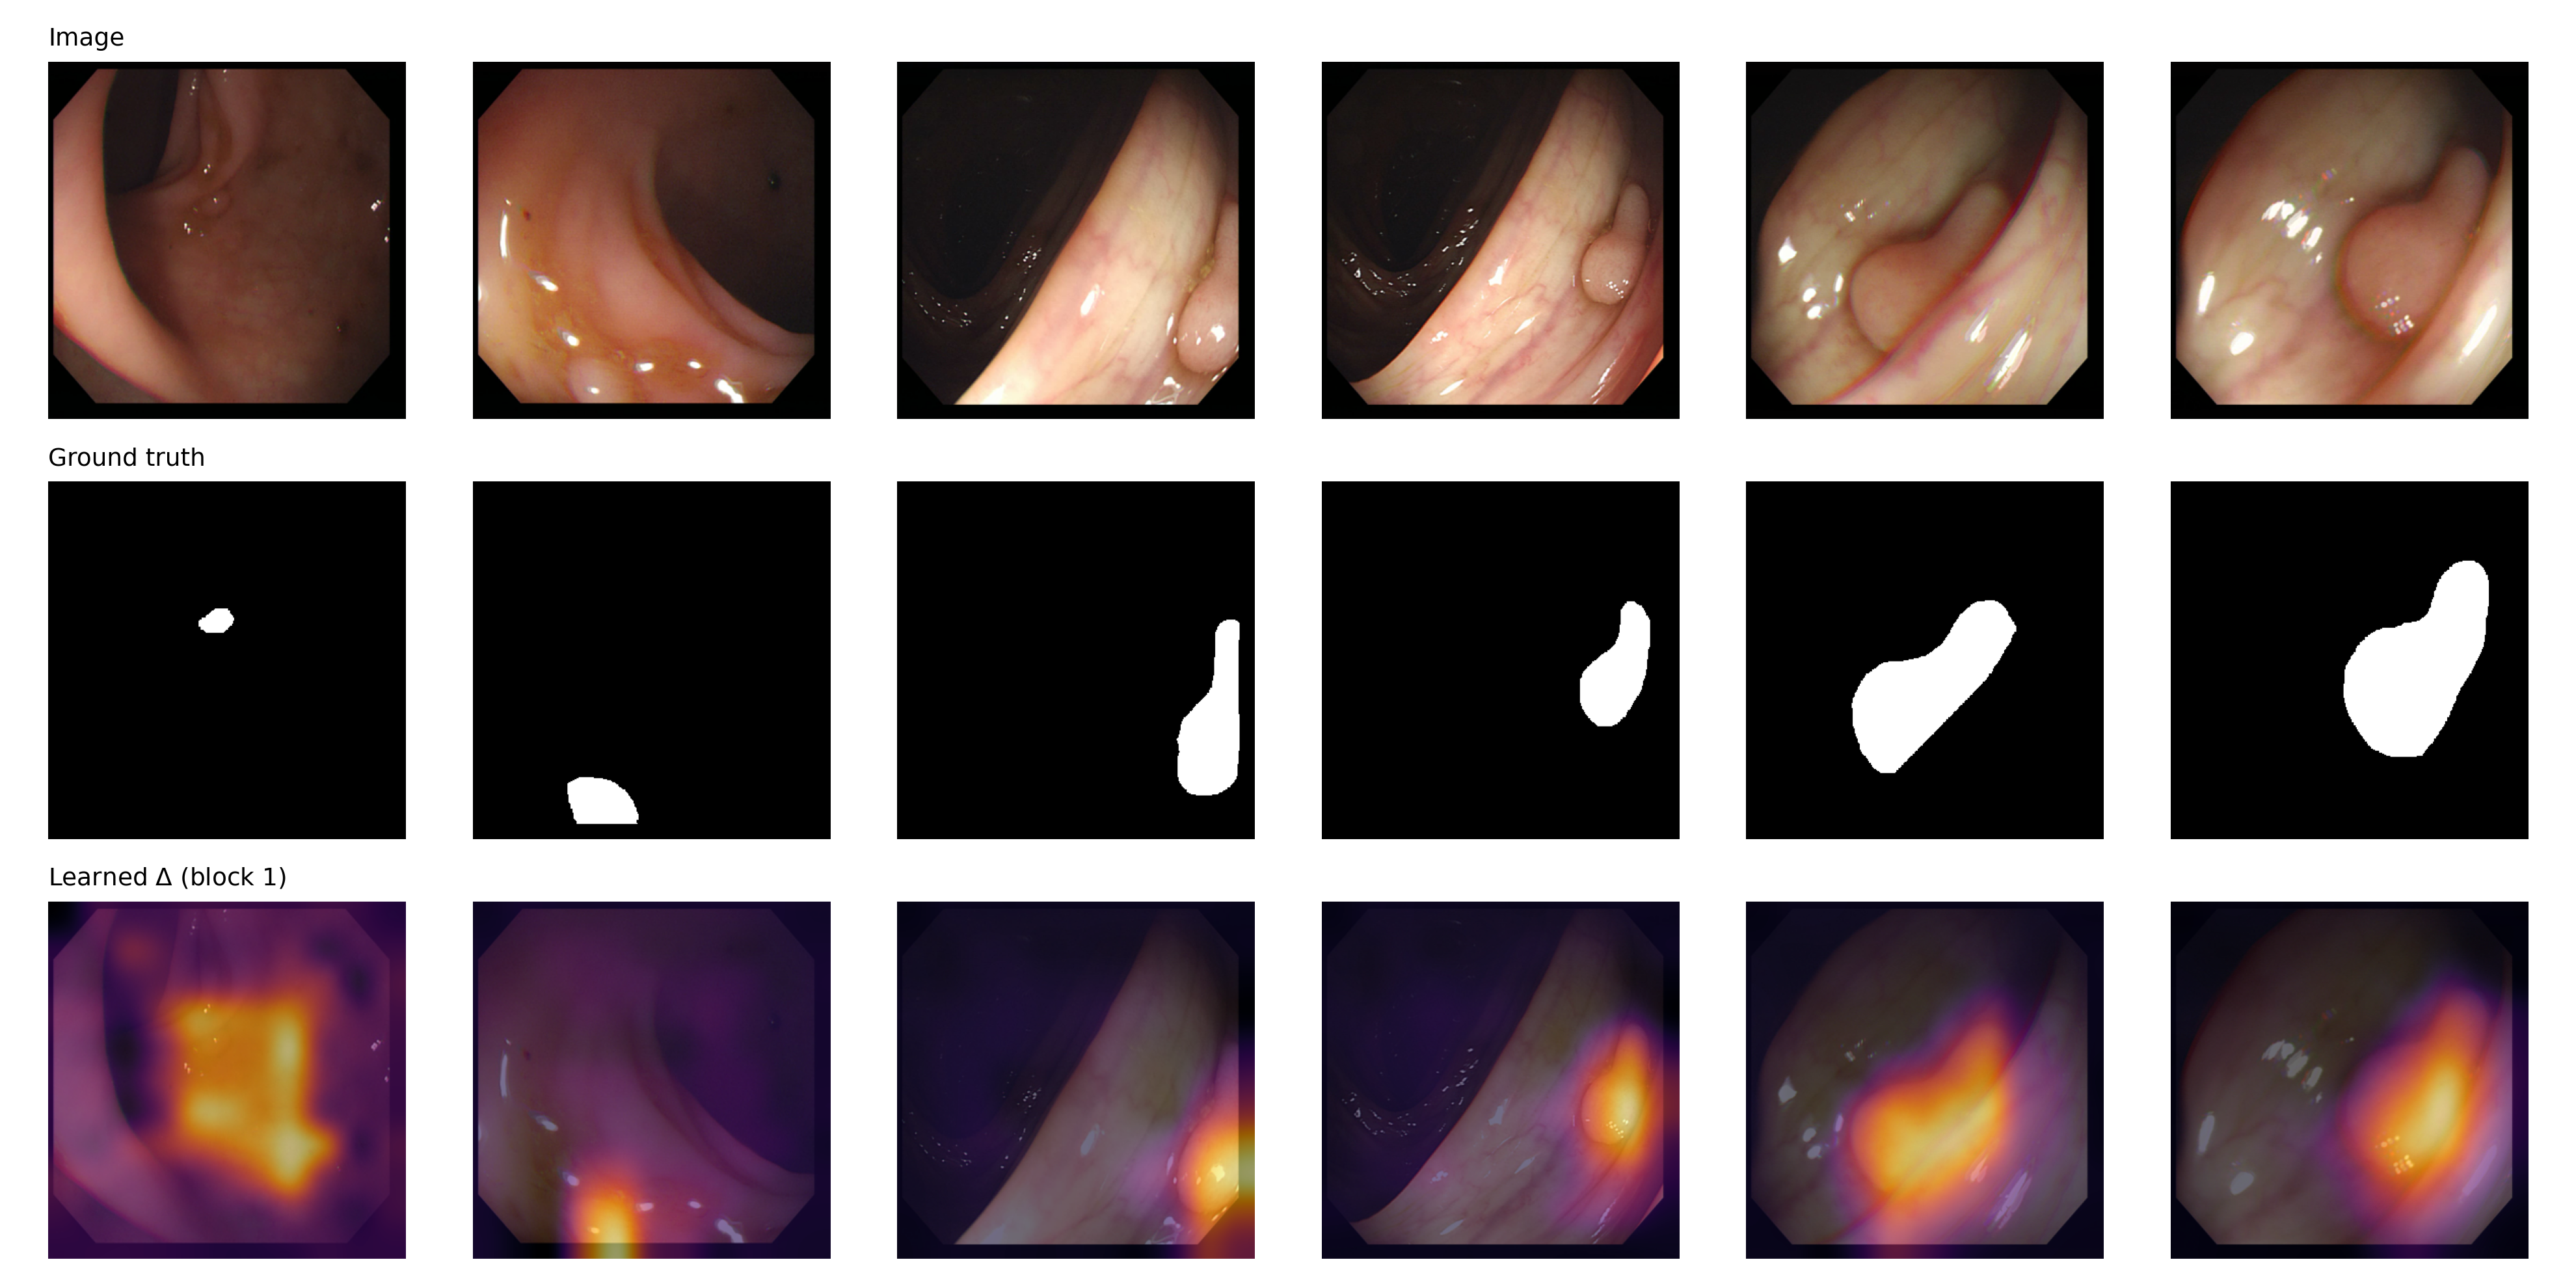
\includegraphics[width=\linewidth]{figures/delta_clean_full_s42.png}}{%
  \fbox{\parbox[c][4cm][c]{0.95\linewidth}{\centering\textcolor{red}{Figure generated by \texttt{analyze\_delta.py}\\(paper/figures/delta\_clean\_full\_s42.png)}}}}
\caption{Learned step-size maps on unseen images (CVC-ColonDB and ETIS). Top: input; middle: ground truth; bottom: $\Dt_t$ of the first BC-SSM block (bright = large step = memory reset), upsampled from the $11\times11$ token grid.}
\label{fig:delta}
\end{figure}

\update{Report Table~\ref{tab:delta} and Fig.~\ref{fig:delta}. If BC-SSM shows a clearly higher ratio and correlation than S6, this is direct evidence for Proposition~\ref{prop:gating}. If not, say so and discuss whether the gain comes mainly through $\vect{B}_t,\vect{C}_t$.}

\subsection{Computational Cost}
\label{sec:cost}
Table~\ref{tab:cost} breaks down the size and cost of B-Mamba. Most of the parameters (86.7\,M) and compute come from the Swin-B encoder. The boundary conditioning itself, which is the subject of this paper, adds only \BCparams\,M parameters and \BCmacs\,GMACs.

\begin{table}[t]
\centering
\caption{Parameters and compute of B-Mamba for one $352\times352$ image. MACs are counted with THOP; FPS is measured with batch size 1.}
\label{tab:cost}
\setlength{\tabcolsep}{5pt}
\begin{tabular}{l r}
\toprule
Component & Params (M) \\
\midrule
Swin-B encoder                          & 86.74 \\
Feature pyramid network                 & 2.85 \\
Boundary Prior Extractor                & 4.99 \\
BC-SSM branch (4 blocks + projections)  & 20.29 \\
\quad of which boundary conditioning    & \BCparams \\
Fusion, input projections               & 0.79 \\
ASPP + progressive decoder              & 5.82 \\
\midrule
\textbf{Total}                          & \textbf{\Params} \\
\midrule
MACs (G)                                & \GMACs \\
\quad of which boundary conditioning    & \BCmacs\ (1.1\%) \\
Inference speed (FPS)                   & \FPS \\
\bottomrule
\end{tabular}
\end{table}

\textbf{SSM versus self-attention.} A common claim is that SSMs are cheaper than Transformers. This is true only when sequences are long, and we want to be precise about it. Table~\ref{tab:scaling} compares one BC-SSM block with one standard Transformer block (multi-head self-attention plus an MLP with ratio 4) of the same width $C=512$, at the token counts that a $352\times352$ image yields at different strides. At stride 32 ($L=121$), where B-Mamba places its SSM, self-attention is actually slightly cheaper (0.40 vs.\ 0.59 GMACs per block); the reason to use an SSM there is its boundary-controllable recurrence, not its speed. The cost curves cross at $L\approx1{,}650$ tokens. At stride 4 ($L=7{,}744$), a BC-SSM block needs 2.3$\times$ fewer MACs than attention, and attention must also store an $L\times L$ score map that grows to 1.8\,GB per block, whereas the SSM state stays at 64\,KB. BC-SSM can therefore be moved to higher-resolution stages, where boundaries are sharper, without a quadratic blow-up; we leave this to future work.

\begin{table}[t]
\centering
\caption{Analytic cost of one token-mixing block (width 512) for a $352\times352$ input at different strides. ``S6'' is the same block without boundary conditioning. Memory is the attention score map (8 heads, fp32) vs.\ the SSM state.}
\label{tab:scaling}
\begin{adjustbox}{max width=\linewidth}
\begin{tabular}{c r c c c r r}
\toprule
\multirow{2}{*}{Stride} & \multirow{2}{*}{$L$} & \multicolumn{3}{c}{GMACs per block} & \multicolumn{2}{c}{Memory} \\
\cmidrule(lr){3-5}\cmidrule(lr){6-7}
 & & S6 & BC-SSM & Attention & Attn.\ map & SSM state \\
\midrule
32 & 121   & 0.45  & 0.59  & 0.40  & 0.4\,MB  & 64\,KB \\
16 & 484   & 1.82  & 2.34  & 1.76  & 7.1\,MB  & 64\,KB \\
8  & 1936  & 7.27  & 9.37  & 9.93  & 114\,MB  & 64\,KB \\
4  & 7744  & 29.09 & 37.46 & 85.77 & 1830\,MB & 64\,KB \\
\bottomrule
\end{tabular}
\end{adjustbox}
\end{table}

\subsection{Qualitative Results}
\begin{figure*}[t]
\centering
\IfFileExists{figures/qualitative.png}{%
  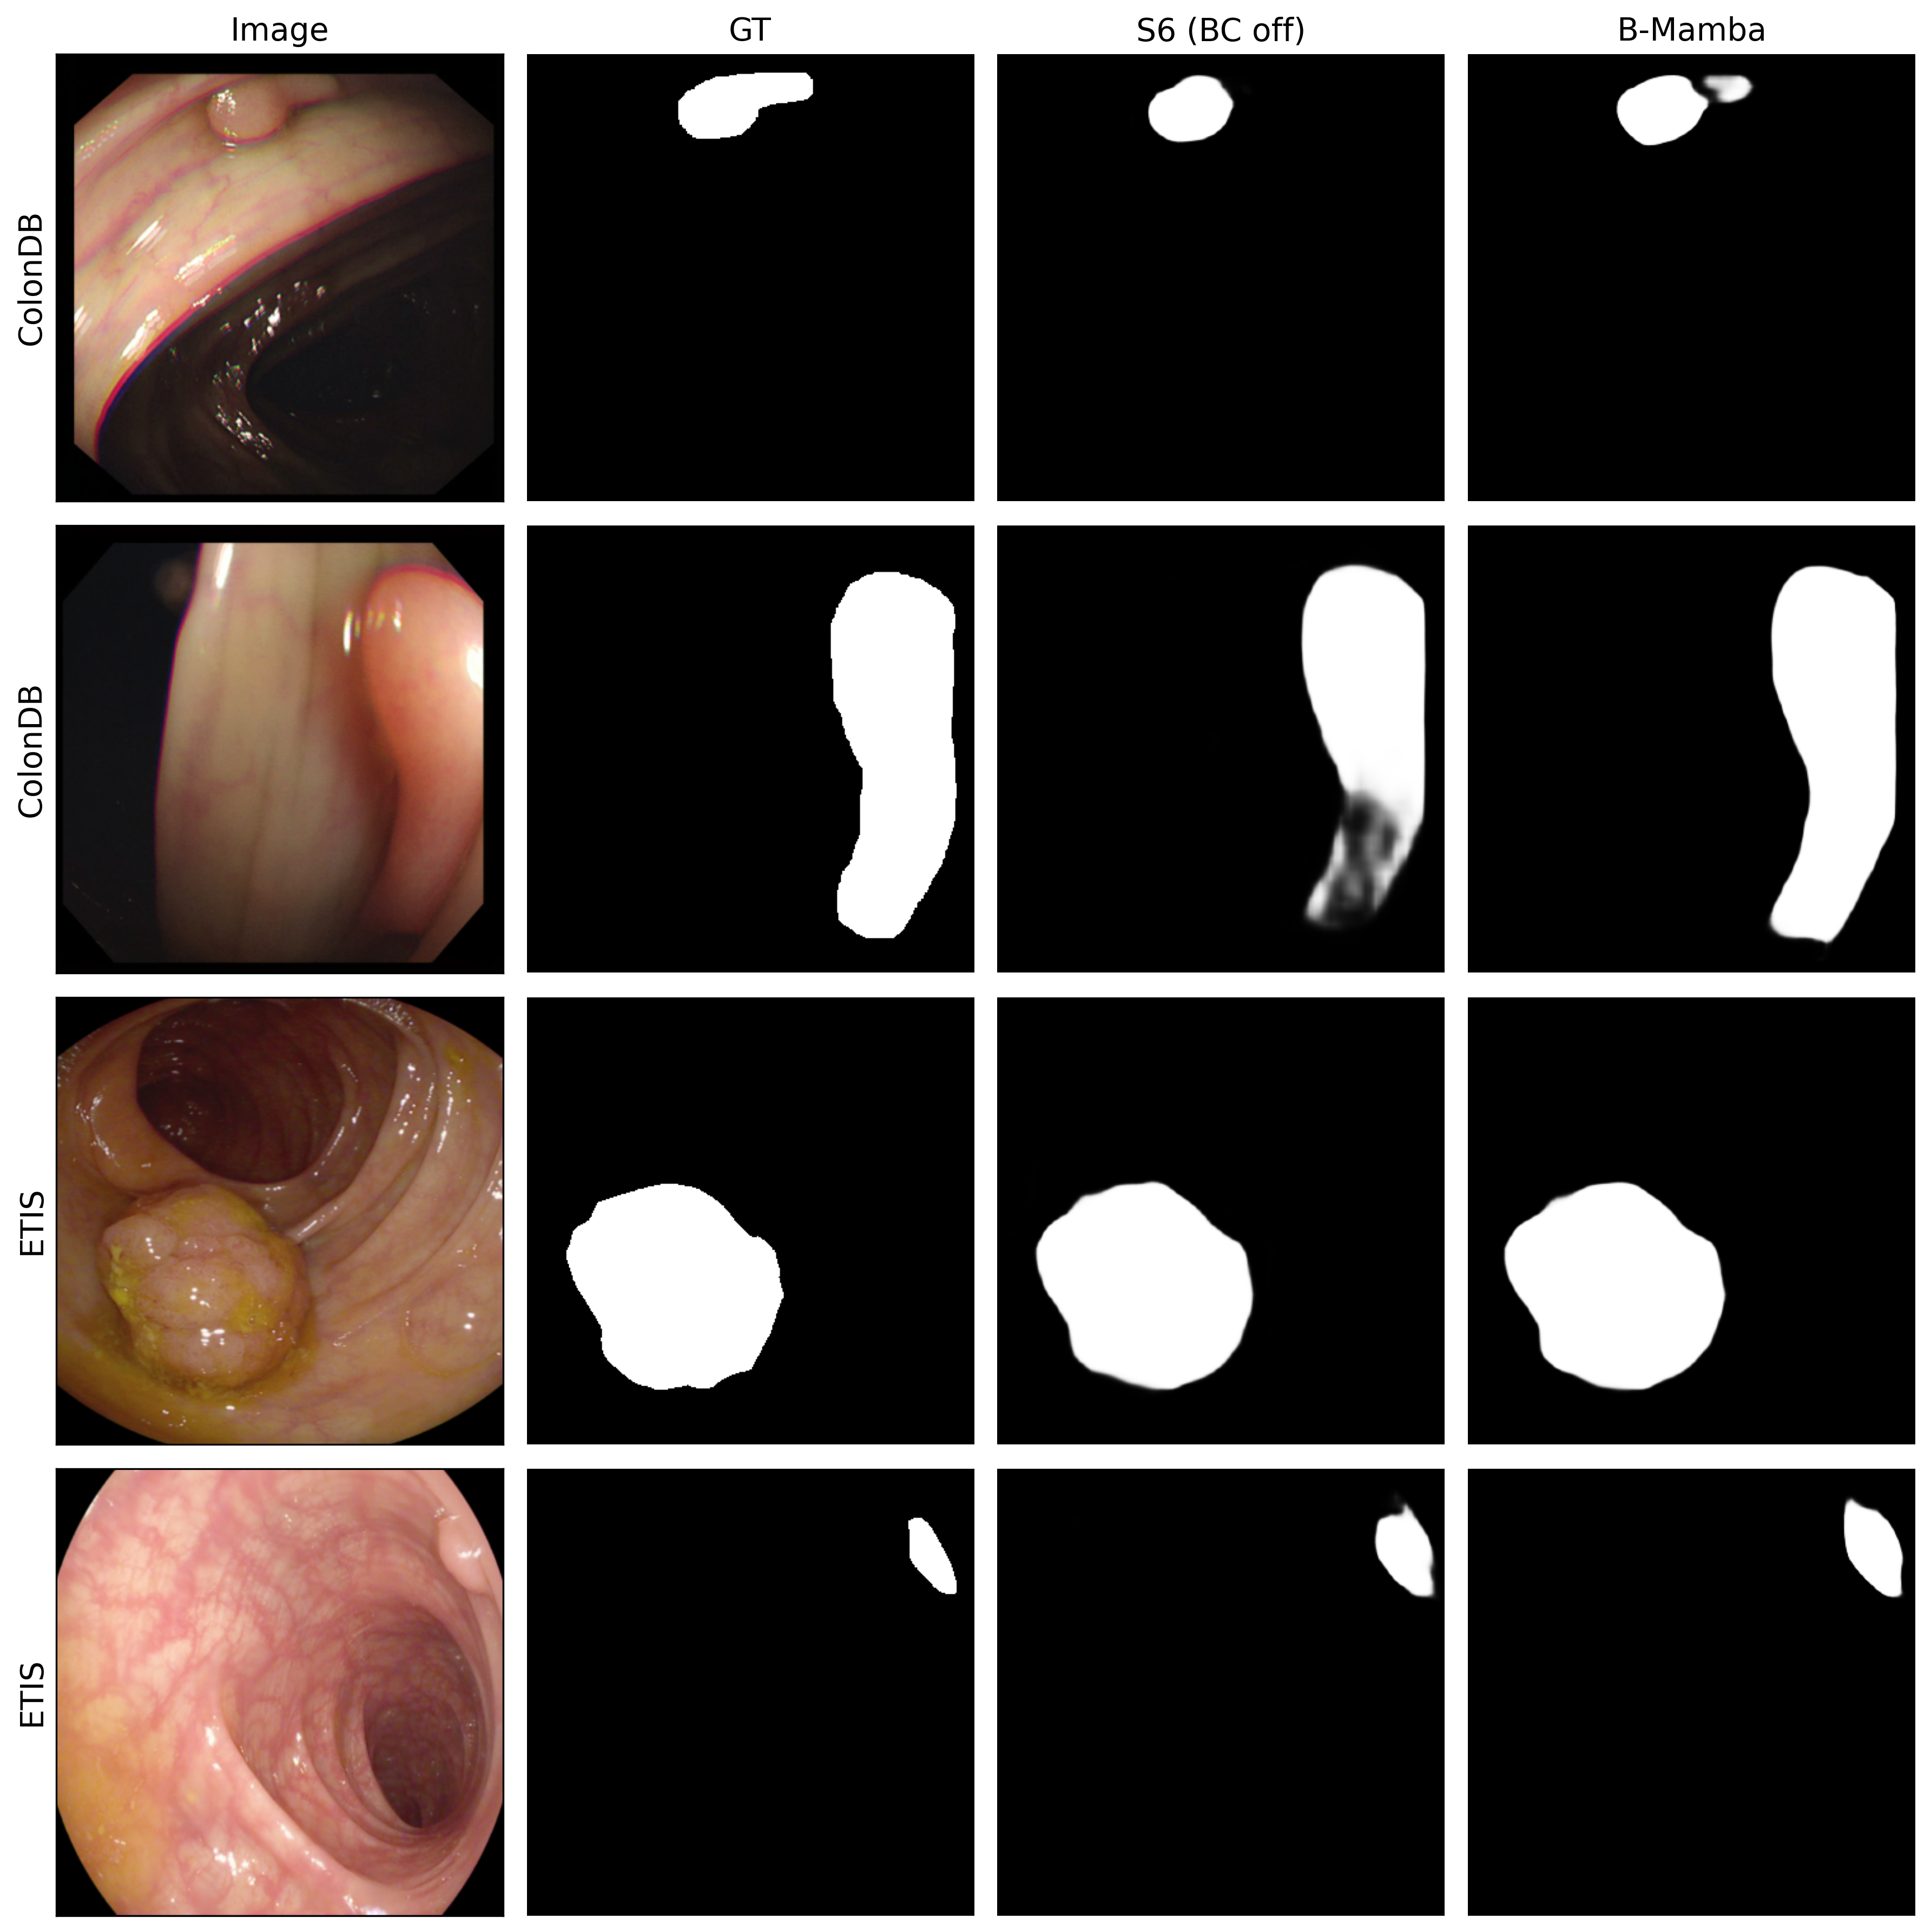
\includegraphics[width=\textwidth]{figures/qualitative.png}}{%
  \fbox{\parbox[c][5cm][c]{0.95\textwidth}{\centering\textcolor{red}{Qualitative comparison on test images (Image / GT / Polyp-PVT / S6 variant / B-Mamba), with weak-boundary cases from ColonDB and ETIS.\\Use test-set images only.}}}}
\caption{Qualitative comparison on challenging test images with weak boundaries, small polyps and specular highlights. Green: ground-truth contour; red: prediction.}
\label{fig:qual}
\end{figure*}

\update{Describe Fig.~\ref{fig:qual}: where B-Mamba follows weak borders better, and also show at least one failure case (e.g., very small flat polyps in ETIS) -- reviewers trust papers that show failures.}

% ==================================================================
\section{Discussion}
\label{sec:discussion}

\textbf{Why condition the dynamics instead of the features?} Adding an edge map to the features, as most boundary-aware networks do, tells the network \emph{that} an edge exists, but leaves it to the following layers to decide what to do with this information. Conditioning the step size tells the sequence model \emph{how to propagate information} around the edge. Propositions~\ref{prop:kernel} and \ref{prop:gating} show that this has a simple and interpretable effect: boundaries become ``long distances'' in the learned metric of the scan. This is also why the change is cheap; it re-uses the selection machinery that Mamba already has.

\textbf{Why a fixed Sobel operator?} A learned edge detector could fit the color statistics of the training hospitals. A fixed gradient operator responds to changes in the features regardless of their absolute values, which we expect to transfer better to new domains. The learned high-frequency branch \eqref{eq:hf} adds flexibility on top of this fixed anchor.

\textbf{Limitations.} We want to be clear about what B-Mamba does not yet do. (1) The BC-SSM operates only at stride 32 ($11\times11$ tokens), where a token covers a large patch; the boundary signal is therefore coarse and fine contours are recovered by the decoder. Table~\ref{tab:scaling} suggests that moving BC-SSM to finer stages is affordable. (2) We use a single raster scan; multi-directional scans \cite{zhu2024vim,liu2024vmamba} could make the boundary effect symmetric. (3) The Sobel prior is computed on the channel mean, which may miss edges that appear in only a few channels. (4) The model is large (121\,M parameters, dominated by the Swin-B encoder) compared with Polyp-PVT (about 25\,M). (5) We evaluate on still images; colonoscopy is a video, and temporal consistency is not modeled. (6) As in all public polyp benchmarks, the test sets are small (60--380 images) and come from a few centers, so prospective clinical validation is still required.

\textbf{Broader applicability.} The BC-SSM is not specific to polyps. Any task where object borders are weak and context matters, such as skin lesions, breast ultrasound or gland segmentation, could use the same block, and the boundary prior could be replaced by any other structural cue (e.g., a depth map or a vessel map).

% ==================================================================
\section{Conclusion}
\label{sec:conclusion}
We introduced B-Mamba, a polyp segmentation network built around a simple observation: the selective state space models used in recent vision networks decide how much context to remember using only local appearance, and so they have no explicit notion of where an object ends. The Boundary-Conditioned SSM fixes this by feeding fixed gradient priors directly into the step size and the input/output matrices of the selective scan. We proved that this strictly generalizes Mamba and that positive boundary responses exponentially limit the flow of information across edges, an edge-aware form of long-range propagation. The conditioning costs about 1\% of the network's compute. Experiments under the leakage-checked five-dataset PraNet protocol, including ablations over three seeds, boundary-specific metrics and a direct analysis of the learned step sizes, \update{summarize final findings}. We hope that conditioning the \emph{dynamics} of sequence models on structural priors will prove useful well beyond polyp segmentation.

% ==================================================================
\bibliographystyle{IEEEtran}
\bibliography{refs}

\end{document}
